\section{Evaluating Belief Apart from Outcome}
\label{sec:evaluation}

\begin{figure}[t]
\centering
\resizebox{\columnwidth}{!}{%
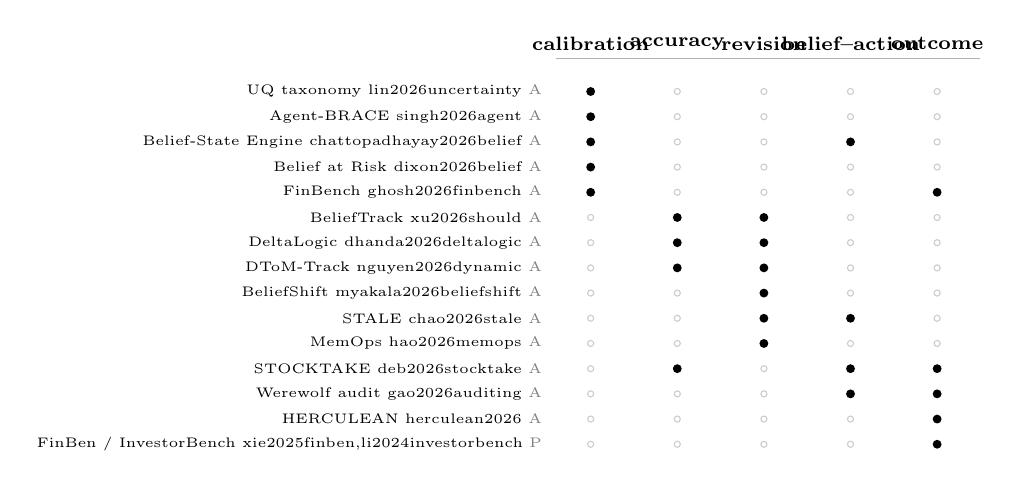
\begin{tikzpicture}[font=\scriptsize, x=11mm, y=3.2mm]
\foreach \c/\x in {calibration/1, accuracy/2, revision/3, belief--action/4, outcome/5} \node[align=center, font=\scriptsize\bfseries, rotate=0] at (\x,0.9) {\c};
\foreach \name/\ev/\y/\dots in {
  {UQ taxonomy \citep{lin2026uncertainty}}/A/-1/{1},
  {Agent-BRACE \citep{singh2026agent}}/A/-2/{1},
  {Belief-State Engine \citep{chattopadhayay2026belief}}/A/-3/{1,4},
  {Belief at Risk \citep{dixon2026belief}}/A/-4/{1},
  {FinBench \citep{ghosh2026finbench}}/A/-5/{1,5},
  {BeliefTrack \citep{xu2026should}}/A/-6/{2,3},
  {DeltaLogic \citep{dhanda2026deltalogic}}/A/-7/{2,3},
  {DToM-Track \citep{nguyen2026dynamic}}/A/-8/{2,3},
  {BeliefShift \citep{myakala2026beliefshift}}/A/-9/{3},
  {STALE \citep{chao2026stale}}/A/-10/{3,4},
  {MemOps \citep{hao2026memops}}/A/-11/{3},
  {STOCKTAKE \citep{deb2026stocktake}}/A/-12/{2,4,5},
  {Werewolf audit \citep{gao2026auditing}}/A/-13/{4,5},
  {HERCULEAN \citep{herculean2026}}/A/-14/{5},
  {FinBen / InvestorBench \citep{xie2025finben,li2024investorbench}}/P/-15/{5}}
 {\node[anchor=east, font=\tiny] at (0.55,\y) {\name~{\color{gray}\ev}};
  \foreach \x in {1,...,5} \draw[gray!40] (\x,\y) circle (1.1pt);
  \foreach \x in \dots \fill (\x,\y) circle (1.6pt);}
\draw[gray!60] (0.6,0.3) -- (5.5,0.3);
\end{tikzpicture}}
\caption{Which belief-level construct each evaluation paper reports. Filled dots mark a reported metric. \textsf{P} = peer-reviewed venue, \textsf{A} = arXiv preprint at the time of writing. No two papers report the same metric for the same construct, which is the fragmentation this section addresses.}
\label{fig:metrics}
\end{figure}


A realised trade or a correct answer can follow from a correct belief, from a wrong belief that did not matter, or from a belief revised too late, and outcome metrics cannot separate the three; this is why stronger backbones do not yield stronger trading agents and the benchmarks cannot say why \citep{xie2025finben,li2024investorbench}. Earlier agent benchmarks score task success or recall \citep{shridhar2020alfworld,liu2023agentbench,maharana2024evaluating,yao2024taubench}; recent work responded with belief-level metrics, each paper defining its own. Figure~\ref{fig:metrics} aligns them by construct, and Table~\ref{tab:benchmarks} in the appendix catalogues 33 benchmarks by whether the evaluator can observe the latent state.

\subsection{Constructs}
\label{sec:eval:constructs}

\emph{Calibration over a trajectory} has the most statistics and the least comparability: checkpoint calibration error, episode-level calibration, posterior entropy, and proper scoring rules on time-gated forecasts express one construct in four ways, none computed on another paper's system \citep{lin2026uncertainty,singh2026agent,chattopadhayay2026belief,dixon2026belief,ghosh2026finbench}. \emph{Belief accuracy and revision} are measured against a known answer in a closed world, after a minimal premise edit, and across recall, inference, and change detection \citep{xu2026should,dhanda2026deltalogic,nguyen2026dynamic}, and against human annotation \citep{myakala2026beliefshift,chao2026stale,hao2026memops,yang2026groupmembench} and, for beliefs about other agents, by theory-of-mind benchmarks \citep{bawatneh2026omnitom,wang2026mindgames}. The \emph{belief--action gap} is the youngest construct: STOCKTAKE scores the agent against an exact Bayes filter on the same observations \citep{deb2026stocktake}, the Werewolf audit reports action--belief consistency \citep{gao2026auditing}, and Agent-ToM monitors an agent's beliefs from its trajectory \citep{ahmed2026agenttom}.

\subsection{Where the Latent State Comes From}
\label{sec:eval:latent}

Every construct beyond calibration needs a latent state to compare against. Controlled environments provide it \citep{deb2026stocktake,xu2026should,alaswad2026why}; long-horizon simulators know it but report belief only through proxies \citep{he2026ycbench,zhang2026retailbenchx,han2026can}; historical replay provides neither, so workflow benchmarks can report a belief failure only at the outcome level \citep{herculean2026}. 

\insight{5}{\textbf{Belief cannot be scored by outcome.} Five constructs, fifteen metrics, no cross-paper comparison; only the fair oracle scores belief and action on the same episodes. Progress on belief will be measurable only where the latent state is known, so controlled environments, not replay, are where the next results should come from.}
